\input{shared/ietf-slides.tex}

% about the presentation
\title{CoAP Transport Indication}
\subtitle{\texttt{ietf-core-transport-indication-09}}
\author{\textit{Christian~Amsüss}, Martine~Lenders}
\date{2025-07-22, CoRE at IETF123 / Madrid}

\begin{document}

\frame{\titlepage}

\begin{frame}{Recap: Mission}\framesubtitle{\footnotesize This slide is getting shorter and shorter per iteration, I think that's good.}\Large
    \begin{itemize}
        \item Consistently address resources without per-transport schemes.
    \end{itemize}
\end{frame}

\begin{frame}{Viewpoint for today}\Large
    If the scheme/authority is insufficient on its own, what helps a client to find the server?

    \vspace{2cm}

    How can a client find a usable proxy?
\end{frame}

\begin{frame}{Parallel perspectives}\Large
    \begin{columns}
        \begin{column}{0.7\textwidth}
            Using web links
           
            \vspace{2cm}

            Using DNS
        \end{column}
        \begin{column}{0.3\textwidth}
            \includegraphics{model-principle.pdf}
        \end{column}
    \end{columns}
\end{frame}

\begin{frame}{Starting point: URI}\Large
    ``You can find the temperature to monitor at the \texttt{/t} of \texttt{sensor1}.''

    \vspace{1cm}

    \texttt{<coap://sensor1.example.com/t>;rt=core.s}

    \vspace{1cm}

    \begin{enumerate}
        \item Where is that?
        \item Which transport can I use?
        \item Which security mechanism should I use?
    \end{enumerate}
\end{frame}

\begin{frame}[fragile]{Where is that?}
    \begin{columns}
        \begin{column}{0.7\textwidth}
\begin{verbatim}
<coap://[2001:db8::1]>;rel=has-proxy;
  anchor="coap://sensor1.example.com"
<coap://[fda9:7eb0:78db::1]>;rel=has-proxy;
  anchor="coap://sensor1.example.com"
\end{verbatim}
% verbose? yes (6690 oddities); core-href is being finished
           
            \vspace{1cm}

\begin{verbatim}
sensor1.example.com IN AAAA 2001:db8::1
sensor1.example.com IN AAAA fda9:7eb0:78db::1
\end{verbatim}
        \end{column}
        \begin{column}{0.3\textwidth}
            \includegraphics{model-aaaa.pdf}
        \end{column}
    \end{columns}
\end{frame}

\begin{frame}[fragile]{Which transports are available?}
    \framesubtitle{TCP version}
    \begin{columns}
        \begin{column}{0.7\textwidth}
\begin{verbatim}
<coap+tcp://[2001:db8::1]>;rel=has-proxy;
  anchor="coap://sensor1.example.com"
\end{verbatim}
           
            \vspace{1cm}

% as mentioned: now using alpn consistently with other non-TLS protocols registered there
\begin{verbatim}
_coap.sensor1.example.com IN SVCB 1 . ( alpn=COAP )
      sensor1.example.com IN AAAA 2001:db8::1
\end{verbatim}
        \end{column}
        \begin{column}{0.3\textwidth}
            \includegraphics{model-tcp.pdf}
        \end{column}
    \end{columns}
\end{frame}

% shown separately to visualize the one thing the coap+ schemes are good for in a world where DNS has SVCB: literals

\begin{frame}[fragile]{Which transports are available?}
    \framesubtitle{over a hypothetical CoAP-over-QUIC}
    \begin{columns}
        \begin{column}{0.7\textwidth}
\begin{verbatim}
<coap://636f7175.alpn.2001-db8--1.6.service.arpa>;
  rel=has-proxy;anchor="coap://sensor1.example.com"
\end{verbatim}
           
            \vspace{1cm}

\begin{verbatim}
_coap.sensor1.example.com IN SVCB 1 . ( alpn=coqu )
      sensor1.example.com IN AAAA 2001:db8::1
\end{verbatim}
        \end{column}
        \begin{column}{0.3\textwidth}
            \includegraphics{model-quic.pdf}
        \end{column}
    \end{columns}
\end{frame}


% for TLS
%
% <coaps+tcp://sensor1.example.com/t>
% 
% <open how to express in link format>\footnote{because the "metadata of the host" was an afterthought in the current design after too much SVCB intake}
% 
% _5684._tcp.sensor1.example.com IN TLSA 3 1 0 hexhexhex

\begin{frame}[fragile]{How do I know whom to talk to?}
    \framesubtitle{Only matters unless there is policy, such as ``we use WebPKI''}
    \begin{columns}
        \begin{column}{0.7\textwidth}
            \vspace{1cm}

\texttt{<coap://hexhexhex.cred.service.arpa/t>}\\
\texttt{<coap+tcp://[2001:db8::1]>;rel=has-proxy;}\\
\texttt{\qquad{}anchor="coap://hexhexhex.cred.service.arpa"}
            \footnote{Questionable name switch, but enables using established sessions.}
           
            \vspace{1cm}

\texttt{\_coap.sensor1.example.com IN SVCB 1 . \textbackslash}\\
\texttt{\qquad{}( alpn="COAP" cred="hexhexhex" )}
            % sorry tex folks, but this *is* just the most discoverable way to make the footnote span both columns
            \footnote{\mbox{DNS gets away without a name switch, but needs DNSSEC to make this really count.}}
            \footnote{What would this look like for an TLSA or SSHFP record? Unsure.}\\
\texttt{sensor1.example.com IN AAAA 2001:db8::1}
            \vspace{1cm}
        \end{column}
        \begin{column}{0.3\textwidth}
          \mbox{}\vspace{-1.5cm}

            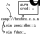
\includegraphics{model-cred-link.pdf}

            \includegraphics{model-cred-svcb.pdf}
        \end{column}
    \end{columns}
\end{frame}

\begin{frame}{Additional notes}\large

    \begin{itemize}
        \item Address of the host? 3rd party proxy? Matters not.
            \bigskip
        \item Non-IP transports are easy (e.\,g. CoAP-over-GATT, slipmux).

          {\footnotesize{Metadata from BLE or USB characteristics.}}
            \bigskip
        \item  Recent changes:
        \begin{itemize}\large
            \item This now states that it is an SVCB mapping document.
            \item \texttt{coaptransport} dissolved into \texttt{alpn}.
            \item Modelling tweaks.
        \end{itemize}
    \end{itemize}
\end{frame}

\begin{frame}{Questions}\framesubtitle{to the WG, unless noted otherwise}\large
    \begin{itemize}
        \item Is the modelling sufficient and suitable?
        \item What are shared properties, what are properties of a transport? % dohpath and TLSA vs ip6hint and alpn

          {\footnotesize In particular, what can we do for the name switch announcing a cryptographic ID?}
        \item Does this fit with the SVCB architecture?

          {\footnotesize Will ask Ben Schwartz for review, whose input from DoC shaped recent changes.}
        \item How does DANE fit SVCB? % different crowds, still all IETF

          {\footnotesize Ask … whom?}
        \item Bikeshedding. (\texttt{.service.arpa}?)
    \end{itemize}
\end{frame}

\end{document}
